% Copyright 2004 by Till Tantau <tantau@users.sourceforge.net>.
%
% In principle, this file can be redistributed and/or modified under
% the terms of the GNU Public License, version 2.
%
% However, this file is supposed to be a template to be modified
% for your own needs. For this reason, if you use this file as a
% template and not specifically distribute it as part of a another
% package/program, I grant the extra permission to freely copy and
% modify this file as you see fit and even to delete this copyright
% notice.

\documentclass[10pt, mathserif, profesionalfont]{beamer}

\usepackage[utf8]{inputenc}
\usepackage[spanish, es-tabla]{babel}

\usepackage[top=3cm,bottom=3cm,outer=2.0cm, inner=3.5cm, marginparwidth = 1.0cm, marginparsep=0.5cm,headsep=10pt, a4paper, heightrounded]{geometry}

\usepackage{amsmath,amsfonts,amssymb,amsthm}
\usepackage{booktabs}
\usepackage{hyperref}
\usepackage{authblk}

\usepackage{empheq}

\usepackage[acronym]{glossaries}

\renewcommand\Affilfont{\itshape\small}
\renewcommand\Authand{ y }

\newtheorem{thm}{Teorema}

\usepackage{array}
\newcolumntype{L}[1]{>{\raggedright\let\newline\\\arraybackslash\hspace{0pt}}p{#1}}
\newcolumntype{C}[1]{>{\centering\let\newline\\\arraybackslash\hspace{0pt}}p{#1}}
\newcolumntype{R}[1]{>{\raggedleft\let\newline\\\arraybackslash\hspace{0pt}}p{#1}}

\newcolumntype{X}[1]{>{\raggedright\let\newline\\\arraybackslash\hspace{0pt}}m{#1}}
\newcolumntype{Y}[1]{>{\centering\let\newline\\\arraybackslash\hspace{0pt}}m{#1}}
\newcolumntype{Z}[1]{>{\raggedleft\let\newline\\\arraybackslash\hspace{0pt}}m{#1}}

\newacronym{ndtm}{NDTM}{Máquina de Turing No Determinista}

\newacronym{sat}{SAT}{SATISFACTIBILIDAD}

\newacronym{3sat}{3SAT}{3-SATISFACTIBILIDAD}




% There are many different themes available for Beamer. A comprehensive
% list with examples is given here:
% http://deic.uab.es/~iblanes/beamer_gallery/index_by_theme.html
% You can uncomment the themes below if you would like to use a different
% one:
%\usetheme{AnnArbor}
%\usetheme{Antibes}
%\usetheme{Bergen}
%\usetheme{Berkeley}
%\usetheme{Berlin}
%\usetheme{Boadilla}
%\usetheme{boxes}
%\usetheme{CambridgeUS}
%\usetheme{Copenhagen}
%\usetheme{Darmstadt}
%\usetheme{default}
%\usetheme{Frankfurt}
%\usetheme{Goettingen}
%\usetheme{Hannover}
%\usetheme{Ilmenau}
%\usetheme{JuanLesPins}
%\usetheme{Luebeck}
\usetheme{Madrid}
%\usetheme{Malmoe}
%\usetheme{Marburg}
%\usetheme{Montpellier}
%\usetheme{PaloAlto}
%\usetheme{Pittsburgh}
%\usetheme{Rochester}
%\usetheme{Singapore}
%\usetheme{Szeged}
%\usetheme{Warsaw}

\title{Teorema de Cook-Levin}

\author{Adrián Rodríguez Bazaga, Eleazar Díaz Delgado, Rudolf Cicko}
% - Give the names in the same order as the appear in the paper.
% - Use the \inst{?} command only if the authors have different
%   affiliation.

\institute[Universidad de La Laguna]{Adrián Rodríguez Bazaga, Eleazar Díaz Delgado \and Rudolf Cicko} % (optional, but mostly needed)

% - Use the \inst command only if there are several affiliations.
% - Keep it simple, no one is interested in your street address.

\date{Complejidad Computacional, Grado en Ingeniería Informática \newline Universidad de La Laguna \newline Curso 2016-2017}
% - Either use conference name or its abbreviation.
% - Not really informative to the audience, more for people (including
%   yourself) who are reading the slides online

\subject{Theoretical Computer Science}
% This is only inserted into the PDF information catalog. Can be left
% out.

% If you have a file called "university-logo-filename.xxx", where xxx
% is a graphic format that can be processed by latex or pdflatex,
% resp., then you can add a logo as follows:

% \pgfdeclareimage[height=0.5cm]{university-logo}{university-logo-filename}
% \logo{\pgfuseimage{university-logo}}

% Delete this, if you do not want the table of contents to pop up at
% the beginning of each subsection:
\AtBeginSubsection[]
{
  \begin{frame}<beamer>{Outline}
    \tableofcontents[currentsection,currentsubsection]
  \end{frame}
}

% Let's get started
\begin{document}

\begin{frame}
  \titlepage
\end{frame}

\begin{frame}{Contenidos}
  \tableofcontents
  % You might wish to add the option [pausesections]
\end{frame}

\section{Introducción}

\begin{frame}{Preámbulo}

\begin{block}{Teorema de Cook: ¿Qué es?}

\end{block}

\end{frame}

\section{Problema de la satisfactibilidad (SAT)}

\begin{frame}{Problema de la satisfactibilidad (SAT)}

\begin{block}{\gls{sat}}
{\small
\noindent ENTRADA: Un conjunto de cláusulas $C=\left \{c_1, c_2, \dots, c_m \right \}$ sobre un conjunto finito $U$ de variables.

\noindent PREGUNTA: ¿Existe una asignación booleana para $U$, tal que satisfaga todas las cláusulas de $C$?
}
\end{block}

\end{frame}

\section{Demostración de la NP-completitud para SAT}

\begin{frame}{SAT es $\mathcal{NP}$-completo I}

  \begin{block}{}
    Primero se demuestra que SAT está en $\mathcal{NP}$. Para ello se puede generar
    una máquina de Turing no determinista(NDTM), que resuelva SAT en tiempo polinomial.
    Es decir, que dada una fórmula booleana $\phi$ se hallen los valores de entrada, tal
    que se satisfaga $\phi$ usando dicha NDTM.
  \end{block}

\end{frame}

\begin{frame}{SAT es $\mathcal{NP}$-completo II}

\begin{block}{}
  Debemos demostrar que para todo lenguaje $L\in \mathcal{NP}$,
  $L \preceq L_{SAT}$.
\end{block}

\begin{block}{}
  Los lenguajes de la clase $\mathcal{NP}$
  son bastante diversos, se trata de una clase infinitamente grande, por lo que
  no esperemos presentar una demostración para cada uno de los lenguajes por
  separado.
\end{block}

\end{frame}


\begin{frame}{SAT es $\mathcal{NP}$-completo III}

\begin{block}{}
  Denotemos por $M$ un programa arbitrario en tiempo polinomial
  para una \gls{ndtm}, especificado por $\Gamma$, $\Sigma$, $b$, $Q$, $q_0$,
  $q_Y$, $q_N$, y $\delta$. Que decide un lenguaje A en un tiempo polinómico
  $n^k$.
\end{block}

\begin{block}{}
  Se representará la $M$ sobre un tablero, en el cual cada fila es representa una configuración:
  \begin{itemize}
  	\item La primera fila representa la configuración inicial de la máquina.
    \item Se acepta el lenguaje si+ alguna fila del tablero es verdadera.
  \end{itemize}
\end{block}

\end{frame}

\begin{frame}{SAT es $\mathcal{NP}$-completo: tabla}

  \begin{figure}[f]
  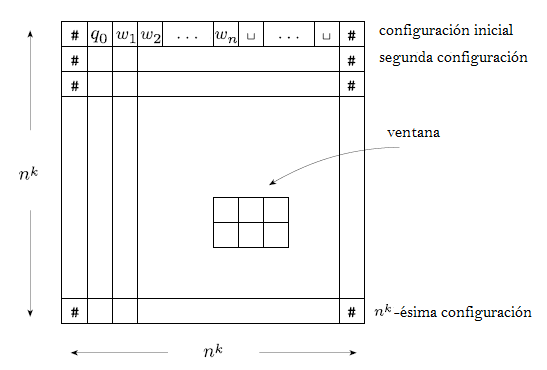
\includegraphics[scale=0.7]{img/1.png}
  \caption{Tabla de configuraciones}
  \end{figure}

\end{frame}

\begin{frame}{SAT es $\mathcal{NP}$-completo IV}

\begin{block}{Generación de la fórmula $\phi$}
  \center{
    $\phi = \phi_{cell} \wedge \phi_{start} \wedge \phi_{move} \wedge \phi_{accept}$}
\end{block}

\end{frame}


\begin{frame}{SAT es $\mathcal{NP}$-completo V}

\begin{block}{Generación de la fórmula $\phi_{cell}$}
  \center{
    $\phi_{cell} = \bigwedge\limits_{1 \le i,j \le n^k} \bigg[\bigg( \bigwedge\limits_{s \in C} x_{i,j,s} \bigg) \wedge \bigg( \bigwedge\limits_{s,t \in C \wedge s \neq t} (\overline{x_{i,j,s}} \lor  \overline{x_{i,j,t}}) \bigg) \bigg]$}
\end{block}

\end{frame}


\begin{frame}{SAT es $\mathcal{NP}$-completo VI}

\begin{block}{Generación de la fórmula $\phi_{start}$}
  \center{
  \begin{equation}
\begin{aligned}
\phi_{start} = {} & x_{1,1,\#} \wedge x_{1,2,q_0} \wedge  \\
      & x_{1,3,w_1} \wedge x_{1,4,w_2} \wedge \dots \wedge x_{1,n+2,w_n} \wedge \\
      &  x_{1,n+3,\textvisiblespace} \wedge \dots \wedge x_{1,n^k-1,\textvisiblespace} \wedge x_{1, n^k,\#}
\end{aligned}
\end{equation}
}
\end{block}

\end{frame}


\begin{frame}{SAT es $\mathcal{NP}$-completo VII}

\begin{block}{Generación de la fórmula $\phi_{accept}$}
  \center{
    $\phi_{accept} = \bigvee\limits_{1 \le i,j \le n^k} x_{i,j,q_{accept}}$}
\end{block}

\end{frame}

\begin{frame}{SAT es $\mathcal{NP}$-completo VIII}

\begin{block}{Generación de la fórmula $\phi_{move}$}
  \center{
    $\phi_{move} = \bigwedge\limits_{1 \le i,j \le n^k} (ventana\ en\ i,j\ que\ es\ legal)$}
\end{block}

\begin{block}{Generación de la fórmula de la ventana}
  \center{
    $\bigvee\limits_{a_1 \dots a_6} x_{i,j-1,a_1} \wedge x_{i,j,a_2} \wedge x_{i,j+1,a_3} \wedge x_{i+1,j-1,a_4} \wedge x_{i+1,j,a_5} \wedge x_{i+1,j+1,a_6}$}
\end{block}

\end{frame}

\section{Conclusiones}

\begin{frame}{Conclusión: SAT es $\mathcal{NP}$-completo}

\begin{itemize}
\item Para todo problema $L$ $\epsilon$ $NP$, existe un $f_L$ que es una transformación polinomial de $L$ al $SAT$
\end{itemize}

\end{frame}

\section{Referencias}

% All of the following is optional and typically not needed. 
\appendix
\section<presentation>*{\appendixname}
\subsection<presentation>*{Referencias}

\begin{frame}[allowframebreaks]
  \frametitle<presentation>{Referencias}
    
  \begin{thebibliography}{10}
    
  \beamertemplatebookbibitems

  \bibitem{Author1990}
    Michael Sipser
    \newblock {\em Introduction to the Theory of Computation}.
    \newblock Third edition, Cengage Learning, 2013
   
  \bibitem{Author1990}
    Michael R. Garey, David S. Johnson
    \newblock {\em Computers and Intractability: A Guide to the Theory of NP-Completeness}.
    \newblock W.H. Freeman. ISBN 0-7167-1045-5.
 
    
  \beamertemplatearticlebibitems

    \bibitem{Someone2000}
    Cook, Stephen
    \newblock {\em The complexity of theorem proving procedures}.
    \newblock Proceedings of t he Third Annual ACM Symposium on Theory of Computing. pp. 151-158 (1971)
    
    \bibitem{Someone2000}
    Karp, Richard M.
    \newblock {\em Reducibility Among Combinatorial Problems}.
    \newblock Complexity of Computer Computations. New York: Plenum, pp. 85-103. ISBN 0-306-30707-3 (1972)
    
    \bibitem{Someone2000}
    T. P. Baker, J. Grill, R. Solovay
    \newblock {\em Relativizations of the P=NP question}.
    \newblock SIAM Journal on Computing. 4 (4): 431-442 (1975)
    
    \bibitem{Someone2000}
    Dekhtiar, M.
    \newblock {\em On the impossibility of eliminating exhaustive search in computing a function relative to its graph}.
    \newblock Proceedings of the USSR Academy of Science. 14: 1146-1148.
    
    \bibitem{Someone2000}
    Levin, Leonid
    \newblock {\em Universal search problems}.
    \newblock Problems of Information Transmission. 9 (3): 115-116 (1973)
    
  \bibitem{Someone2000}
    Design and Analysis of Algorithms
    \newblock {\em Lecture, School of Information and Computer Sciences, University of California, Irvine}
    \newblock \url{https://www.ics.uci.edu/~eppstein/161/960312.html}
    
  \bibitem{Someone2000}
    NP-complete problems
    \newblock {\em Lecture, Electrical Engineering and Computer Sciences, Berkeley}
    \newblock \url{https://people.eecs.berkeley.edu/~vazirani/algorithms/chap8.pdf}
  \end{thebibliography}
\end{frame}

\end{document}
